\pagebreak
\subsection{Thermal Design} \label{Thermal_section}

\subsubsection{Thermal Environment}
\begin{centering}
The experiment will experience wide temperature fluctuations during the flight and it must be able to continue to operate despite these changes. As seen in Figure \ref{fig:temperature-profile} the coldest point of the flight will be between 10 km and 15 km where the air temperature can drop to $-80\degree$ C outside. Past flights have recorded temperatures on the gondola as low as $-40\degree$ C during the Float Phase\cite{BexusManual}. Sampling with the AAC will begin when the balloon has risen to 18 km during the Ascent Phase and will last until the Float Phase. Sampling will resume when the gondola has fallen to 19 km during the Descent Phase. This means the experiment will be above the coldest part of the atmosphere and the critical components will have time to achieve their operating temperature before sampling time commences. In addition, launching from Kiruna in late October means the temperature on the ground could be as low as $-10\degree$ C. 
As the component with the highest lower limit operating temperature must be at a minimum of $5\degree$ C (E3 in Table \ref{tab:thermal-table}), heating may need to be switched on while the experiment is still on the ground.
\end{centering}

\begin{figure}[H]
    \begin{align*}
        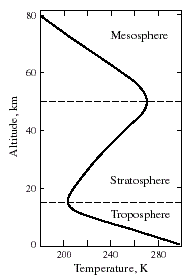
\includegraphics[height=8cm]{4-experiment-design/img/temperature-profile.png}
    \end{align*}
    \caption{Diagram Showing the Temperature Profile of the Atmosphere \cite{jacob}}\label{fig:temperature-profile}
\end{figure}

\subsubsection{The Critical Stages}
The flight will have the following critical stages:
\begin{itemize}
    \item Launch pad
    \item Early ascent
    \item Sampling ascent
    \item Float
    \item Descent before sampling
    \item Sampling descent
    \item Shut down
    \item Landed, waiting for recovery
\end{itemize}
These stages have been accounted for in further calculations and simulations.

\subsubsection{Overall Design}
To protect the components against the cold, thermal protection will need to be designed. Insulation and internal heating will both come into play in keeping all the components functional throughout the duration of the flight. The two components with the most critical thermal ranges are the pump and the valve manifold system (E3 and E5 in Table \ref{tab:thermal-table}). Thermal regulation is mainly focused on the AAC however, a thermal analysis of the CAC can be found in Appendix \ref{sec:appI} under section \ref{sssec:CAC-trial-flight} where the  CAC box the valve is identified as the critical component in terms of thermal regulation (refer to component E5 in Table \ref{tab:thermal-table}). It will have a current through it through out the flight heating it self up.

% New for the SED v2
The main protection against the cold environment in the stratosphere is a passive thermal design by means of  insulating layers added to the walls of the experiment. It will be comprised of two layers: one outer sheet of aluminum and a thicker sheet of Styrofoam. The main insulating factor is the 20 mm thick Styrofoam which will significantly reduce the heat exchange between the otherwise exposed experiment box, and will also provide shock absorption when the gondola lands after separating from the balloon.

\begin{figure}[H]
    \centering
    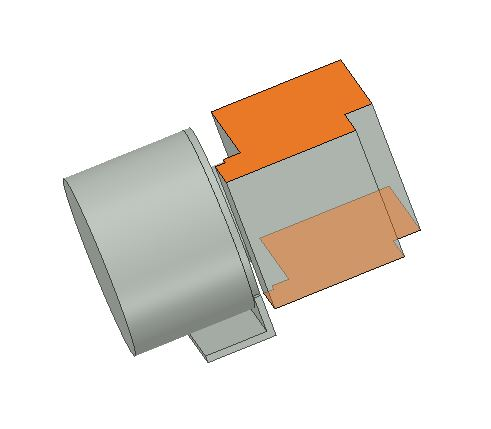
\includegraphics[width=0.5\linewidth]{4-experiment-design/img/Thermal/higlighted-heater-pump.JPG}
    \caption{Highlight of the Heater On the Pump}
    \label{fig:highlight-heater-on-pump}
\end{figure}

An active thermal control system will also be included consisting of three heaters. Two heaters will regulate the pump's temperature as seen in Figure \ref{fig:highlight-heater-on-pump} and a single heater will regulate the valve manifold temperature. To control these heaters, two temperature sensors will also be on board in close proximity to the heaters. If the reading from one of the temperature sensors is lower than the predefined threshold, then the heater will turn on to warm up the cooling component. If it is above the higher threshold the heater will turn off.

Simulation in MATLAB (code can be found in Appendix \ref{sec:appJ}) where used to determine the uniform heat inside the experiment. The ANSYS thermal modelling platform was used to the simulate the thermal conditions inside the Brain.

Table {\ref{tab:thermal-table}}, below, covers the thermal ranges of the components listed in Section \ref{sec:experiment-components}:



%Added this space to help us see all of the numbers. This "Track changes" sign blocks them every time!


\begin{longtable}{|m{1cm}|m{3.5cm}|m{1.3cm}|m{1.3cm}|m{1.4cm}|m{1.3cm}|m{1.3cm}|m{1.3cm}|}
\hline
\multirow{2}{*}{\textbf{ID}} & \multirow{2}{*}{\textbf{Components}}                                 & \multicolumn{2}{l|}{\textbf{Operating (°C)}} & \multicolumn{2}{l|}{\textbf{Survivable (°C)}} & \multicolumn{2}{l|}{\textbf{Expected (°C)}} \\ \cline{3-8} &   & Min.  & Max.  & Min.  & Max.  &  Min.   &  Max.            \\ \hline
E1 & Arduino Due & -40 & 85 & -60 & 150 & -30.62 & 24.01 \\ \hline
E2 & Ethernet Shield & -40 & 85 & -65 & 150 & -30.62 & 24.01 \\ \hline
E3 & Miniature diaphragm air pump & 5 & 40 & -10 & 40 & 10 & 34.93 \\ \hline
E4 & Pressure Sensor & -40 & 85 & -40 & 125 & -19.70 & 34.93 \\ \hline
E5 & Sampling Valve (inlet and outlet 1/8"" female) & -20 & 50 & -20\footnote{If survivable temperatures were not given, operating temperatures were used as survivable limits.\label{fn:erik}} & 50\textsuperscript{\ref{fn:erik}} & -15 & 20 \\ \hline
E6 & Airflow sensor AWM43300V & -20 & 70 & -20\textsuperscript{\ref{fn:erik}} & 70\textsuperscript{\ref{fn:erik}} & -8.77 & 34.93 \\ \hline
E7 & Heater ($12.7\times 50.8 mm$) & -200 & 200 & -200\textsuperscript{\ref{fn:erik}} & 200\textsuperscript{\ref{fn:erik}} & -20 & 36 \\ \hline
E8 & Voltage Regulator & -40 & 125 & -40\textsuperscript{\ref{fn:erik}} & 125\textsuperscript{\ref{fn:erik}} & -30.62 & 34.93 \\ \hline
E9 & Temperature Sensor & -55 & 125 & -65 & 150 & -19.70 & 34.93 \\ \hline
E10 & DCDC 24 V & -40 & 85 & -55 & 125 & -19.70 & 34.93 \\ \hline
E12 & Micro SD & -25 & 85 & -200\textsuperscript{\ref{fn:erik}} & 200\textsuperscript{\ref{fn:erik}} & -19.70 & 34.93 \\ \hline
% E13 & Logic CAT5E & -20 & 75 & (-20)\textsuperscript{\ref{fn:erik}} & (75)\textsuperscript{\ref{fn:erik}} & TBD\textsuperscript{\ref{fn:ivan}} & TBD\textsuperscript{\ref{fn:ivan}} \\ \hline
% E14 & Resistors (33, 150 and 100 ohm) & -55 & 155 & (-55)\textsuperscript{\ref{fn:erik}} & (155)\textsuperscript{\ref{fn:erik}} & TBD\textsuperscript{\ref{fn:ivan}} & TBD\textsuperscript{\ref{fn:ivan}} \\ \hline
% E15 & Capacitors $(0.1 \mu$ F and $10 \mu$ F) & -30 & 85 & (-200)\textsuperscript{\ref{fn:erik}} & (200)\textsuperscript{\ref{fn:erik}} & TBD\textsuperscript{\ref{fn:ivan}} & TBD\textsuperscript{\ref{fn:ivan}} \\ \hline
E16 & Mosfet for current control & -55 & 175 & -55 & 175 & -20 & -20 \\ \hline
E17 & Diodes for DCDC converters & -65 & 175 & -65\textsuperscript{\ref{fn:erik}} & 175\textsuperscript{\ref{fn:erik}} & -19.70 & 34.93 \\ \hline
E18 & 3.3V LED & -40 & 85 & -40\textsuperscript{\ref{fn:erik}} & 85\textsuperscript{\ref{fn:erik}} & -19.70 & 24.01 \\ \hline 
E19 & 15-pin D-SUB Female connector with pins & -55 & 120 & -200\textsuperscript{\ref{fn:erik}} & 200\textsuperscript{\ref{fn:erik}} & -8.77 & 24.01 \\ \hline
E20 & 9-pin D-SUB Female connector with pins & -55 & 120  & -200\textsuperscript{\ref{fn:erik}} & 200\textsuperscript{\ref{fn:erik}} & -8.77 & 24.01 \\ \hline
E21 & 9-pin D-SUB Female connector with soldering cups & -55 & 105 & -55\textsuperscript{\ref{fn:erik}} & 105\textsuperscript{\ref{fn:erik}} & -8.77 & 24.01 \\ \hline
E22 & 9-pin D-SUB Male connector with soldering cups & -55 & 105 & -55\textsuperscript{\ref{fn:erik}} & 105\textsuperscript{\ref{fn:erik}} & -8.77 & 24.01 \\ \hline
E23 & 15-pin D-SUB Male connector with soldering cups & -55  & 105 & -55\textsuperscript{\ref{fn:erik}} & 105\textsuperscript{\ref{fn:erik}} & -8.77 & 24.01 \\ \hline
E24 & 9-pin D-SUB backing & -40 & 120 & -40\textsuperscript{\ref{fn:erik}} & 120 & -8.77 & 24.01  \\ \hline
E25 & 15-pin D-SUB backing & -40 & 120 & -40\textsuperscript{\ref{fn:erik}} & 120 & -8.77 & 24.01  \\ \hline
% E26 & Wall mounting bolts & TBD\textsuperscript{\ref{fn:ivan}} & TBD\textsuperscript{\ref{fn:ivan}} & TBD\textsuperscript{\ref{fn:ivan}} & TBD\textsuperscript{\ref{fn:ivan}} & TBD\textsuperscript{\ref{fn:ivan}} & TBD\textsuperscript{\ref{fn:ivan}} \\ \hline
E27 & D-SUB cable CAC to AAC & -40 & 85 & -55 & 125 & -40 & 40 \\ \hline
% E28 & 3.3 Zener diode & TBD\textsuperscript{\ref{fn:ivan}} & 175 & TBD\textsuperscript{\ref{fn:ivan}} & (175)\textsuperscript{\ref{fn:erik}} & TBD\textsuperscript{\ref{fn:ivan}} & TBD\textsuperscript{\ref{fn:ivan}} \\ \hline
E29 & Male connector on PCB & -40 & 85 & -40\textsuperscript{\ref{fn:erik}} & 85 & -8.77 & 24.01 \\ \hline
E30 & Female connector from wall & -40 & 85 & -40\textsuperscript{\ref{fn:erik}} & 85 & - & - \\ \hline
% E31 & Grounding contact & -55 & 125 & (-55)\textsuperscript{\ref{fn:erik}} & (125)\textsuperscript{\ref{fn:erik}} & TBD\textsuperscript{\ref{fn:ivan}} & TBD\textsuperscript{\ref{fn:ivan}} \\ \hline
E32 & Logic CAT5 E-link for inside box &-20 & 75 & -20\textsuperscript{\ref{fn:erik}} & 75\textsuperscript{\ref{fn:erik}} & -15 & 20 \\ \hline
E33 & Signal Wires & -60 & 200 & -60\textsuperscript{\ref{fn:erik}} & 200\textsuperscript{\ref{fn:erik}} & - & - \\ \hline
E34 & Flushing valve (inlet and outlet 1/8"" female) & -10 & 50 & -10\textsuperscript{\ref{fn:erik}} & 50\textsuperscript{\ref{fn:erik}} & -7.36 & 42.53 \\ \hline
E35 & Valves manifold (outlet 1/8"" female) & -10 & 50 & -10\textsuperscript{\ref{fn:erik}} & 50\textsuperscript{\ref{fn:erik}} & -6.77 & 40.504 \\ \hline
E36 & Power wire black & -60 & 200 & -60\textsuperscript{\ref{fn:erik}} & 200\textsuperscript{\ref{fn:erik}} & - & - \\ \hline
% E37 & Electrical Tape for marking wires (White) & -10 & 90 & (-10)\textsuperscript{\ref{fn:erik}} & (90)\textsuperscript{\ref{fn:erik}} & TBD\textsuperscript{\ref{fn:ivan}} & TBD\textsuperscript{\ref{fn:ivan}} \\ \hline
% E38 & Electrical Tape for marking wires (Black) & -10 & 90 & (-10)\textsuperscript{\ref{fn:erik}} & (90)\textsuperscript{\ref{fn:erik}} & TBD\textsuperscript{\ref{fn:ivan}} & TBD\textsuperscript{\ref{fn:ivan}} \\ \hline
% E39 & Electrical Tape for marking wires (Green) & -10 & 90 & (-10)\textsuperscript{\ref{fn:erik}} & (90)\textsuperscript{\ref{fn:erik}} & TBD\textsuperscript{\ref{fn:ivan}} & TBD\textsuperscript{\ref{fn:ivan}} \\ \hline
% E40 & Electrical Tape for marking wires (Violet) & -10 & 90 & (-10)\textsuperscript{\ref{fn:erik}} & (90)\textsuperscript{\ref{fn:erik}} & TBD\textsuperscript{\ref{fn:ivan}} & TBD\textsuperscript{\ref{fn:ivan}} \\ \hline
% E41 & Electrical Tape for marking wires (Gray) & -10 & 90 & (-10)\textsuperscript{\ref{fn:erik}} & (90)\textsuperscript{\ref{fn:erik}} & TBD\textsuperscript{\ref{fn:ivan}} & TBD\textsuperscript{\ref{fn:ivan}} \\ \hline
% E42 & Electrical Tape for marking wires (Brown) & -10 & 90 & (-10)\textsuperscript{\ref{fn:erik}} & (90)\textsuperscript{\ref{fn:erik}} & TBD\textsuperscript{\ref{fn:ivan}} & TBD\textsuperscript{\ref{fn:ivan}} \\ \hline
% E43 & Electrical Tape for marking wires (Blue) & -10 & 90 & (-10)\textsuperscript{\ref{fn:erik}} & (90)\textsuperscript{\ref{fn:erik}} & TBD\textsuperscript{\ref{fn:ivan}} & TBD\textsuperscript{\ref{fn:ivan}} \\ \hline
% E44 & Heat shrinking tube 2.5 x 1mm & -55 & 125 & (-55)\textsuperscript{\ref{fn:erik}} & (125)\textsuperscript{\ref{fn:erik}} & TBD\textsuperscript{\ref{fn:ivan}} & TBD\textsuperscript{\ref{fn:ivan}} \\ \hline
E45 & 25-pin D-SUB female connector with pins & -10 & 90 & -10\textsuperscript{\ref{fn:erik}} & 90\textsuperscript{\ref{fn:erik}} & -8.77 & 24.01 \\ \hline
E46 & 25-pin D-SUB male connector with soldering cups & -10 & 90 & -10\textsuperscript{\ref{fn:erik}} & 90\textsuperscript{\ref{fn:erik}} & -8.77 & 24.01 \\ \hline
E47 & 25-pin D-SUB backing & -10 & 90 & -10\textsuperscript{\ref{fn:erik}} & 90\textsuperscript{\ref{fn:erik}} & -8.77 & 24.01 \\ \hline
E48 & Power wire red & -60 & 200 & -60\textsuperscript{\ref{fn:erik}} & 200
\textsuperscript{\ref{fn:erik}} & - & -  \\ \hline
% E49 & Potentiometer 1k ohm & -55 & 125 & (-55)\textsuperscript{\ref{fn:erik}} & (120)\textsuperscript{\ref{fn:erik}} & TBD\textsuperscript{\ref{fn:ivan}} & TBD\textsuperscript{\ref{fn:ivan}} \\ \hline
E50 & 6-pin male & -55 & 105 & -55\textsuperscript{\ref{fn:erik}} & 105\textsuperscript{\ref{fn:erik}} & -8.77 & 24.01  \\ \hline
E51 & 8-pin male single row header& -40 & 105 & -40\textsuperscript{\ref{fn:erik}} & 105\textsuperscript{\ref{fn:erik}} & -8.77 & 24.01  \\ \hline
E52 & 10-pin male single row header & -55 & 105 & -55\textsuperscript{\ref{fn:erik}} & 105\textsuperscript{\ref{fn:erik}} & -8.77 & 24.01  \\ \hline
E53 & 36-pin male double row header & -40 & 105 & -40 & 125 & -8.77 & 24.01  \\ \hline
E54 & 12 V DC/DC converter & -40 & 85 & -55 & 125 & -8.77 & 24.01  \\ \hline
E56 & Pressure Sensor & -40 & 120 & -40\textsuperscript{\ref{fn:erik}} & 120\textsuperscript{\ref{fn:erik}} &  -8.77 & 34.93 \\ \hline


\caption{Table of Component Temperature Ranges.}
\label{tab:thermal-table}
\end{longtable}
\raggedbottom










\raggedbottom

\subsubsection{Internal Temperature}
As the current experiment model stands, an enclosed partition has been reserved in the lower front left-hand corner of the AAC section of the experiment. This partition will house all of the electronic components not required to be situated in specified locations throughout the experiment setting, such as some of the sensors.

The pump has the most critical temperature range as it is a single point of failure component that cannot operate below freezing temperatures. It's data sheet states that it must always operate above $5\degree$ C, or the EPDM diaphragm may not be able to expand and contract sufficiently to maintain the desired airflow of 8 L/min. However, as this pump has been used successfully on previous high altitude flights, \cite{LISA}, tests will be conducted on the pump to find its true performance at lower temperatures and low vacuum environment. The AAC valves are also crucial to the experiment's function, as they enable each and every sampling bag on board to be used. For this reason, while the valves can operate down to $-20\degree$ C, it is desirable to be keep them above this limit whenever in use.

As the most temperature-sensitive equipment will all be housed within the Brain, it is important to know what heat will be lost through the different heat transfer mechanisms as this will affect the amount of time the heaters will need to be active. This has been addressed through calculations and simulations to find required insulation. All calculations concerning heat transfer can be found in Appendix \ref{sec:appI}. As a worst-case scenario for heat distribution, it is assumed that \textit{all} of the power dissipated through resistance in the electrical components will reach the marked boundaries of the experiment's walls.

Aluminum sheeting will be used as the outer layer of insulation for the experiment and Styrofoam brand foam will be used as the inner layer. Aluminum may have among the highest of thermal conductivities, but its arrangement around the Styrofoam, creating one large heat bridge with the inner layer, would provide a useful thermoregulatory mechanism \cite{EngTool}. The high ratio between the absorptivity (0.3) and emissivity (0.09) of the material may be used to its advantage \cite{EngTool}. Because the ratio for polished aluminum is higher than 1.0, the element will get hotter as it gets exposed to the radiation from the sun and the power-dissipating components \cite{RedRok}. The low emissivity coefficient for the aluminum cover means it will not get significantly hotter than the surrounding ambient temperature, but its increased temperature may negate some of the heat being lost from the experiment's interior via some of the heat from the aluminum propagating into the experiment, reducing the net heat loss by a small amount. As conservation of power is imperative, the heaters should be used sparingly, and instead methods like the use of aluminum for shielding should be employed as passive heating. The aluminum layer will be 0.5 mm in thickness, while the Styrofoam layer beneath it would span 20 mm in thickness. The Styrofoam, in contrast to the aluminum has a low thermal conductivity even when compared to similar polymer structures \cite{EngTool}. The Styrofoam would handle the bulk of the thermal resistance in keeping the experiment from losing the heat it would have obtained prior to being moved to the launchpad. The aluminum would come into play as the experiment rises into colder altitudes and encounters increased sun exposure. While the warmed aluminum will have little impact on the experiment's heat loss, this also means that the experiment's internal temperatures will be prevented from rising to the upper allowed operating limit of the experiment made possible because of the aluminum's low absorptivity of sunlight.


\subsubsection{Calculations and Simulation Reports}
\label{sec:4.6.5}

The temperature ranges can vary for the different stages but the most critical moment is during the Ascent Phase. While ascending, the main source of heat to maintain the pump and manifold's operating temperature is the heaters. During the Float and Descent Phases, heat originating from the sun will be enough to maintain these component's operational temperatures. According to the thermal analysis, the heaters would not be required during descent but there is power reserved in the worst case scenario that they need to be run during the Descent Phase.
All simulation equations and their details can be seen in Appendix \ref{sec:appI}. 

An estimate of the temperature in the Brain at the sampling times during the Ascent Phase is visualized in Figure \ref{fig:Air-in-brain-4-6}. The higher temperature is in the lower left corner where the pump is located. A cooler area exists around the middle of the right edge where the pipe from the manifold leads to the outside of the experiment. The legend in the Figure shows the temperature in Celsius.

\begin{figure}[H]
    \centering
    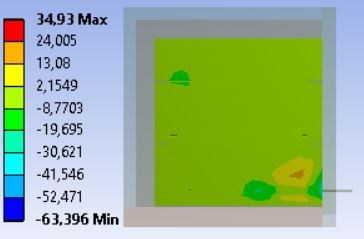
\includegraphics[width=0.7\textwidth]{4-experiment-design/img/Thermal/air-sampling-with-box}
    \caption{Cross Section of the Air in the Brain at the Time to Start Sample During Ascent}
    \label{fig:Air-in-brain-4-6}
\end{figure}

A MATLAB simulated test flight is presented in Figure \ref{fig:test-flight-AAC-4-6}. The blue line is the temperature of the uniform inside air temperature in the AAC experiment box. The BEXUS 25 flight data is the ambient temperature of the outside air.
\begin{figure}[H]
    \centering
    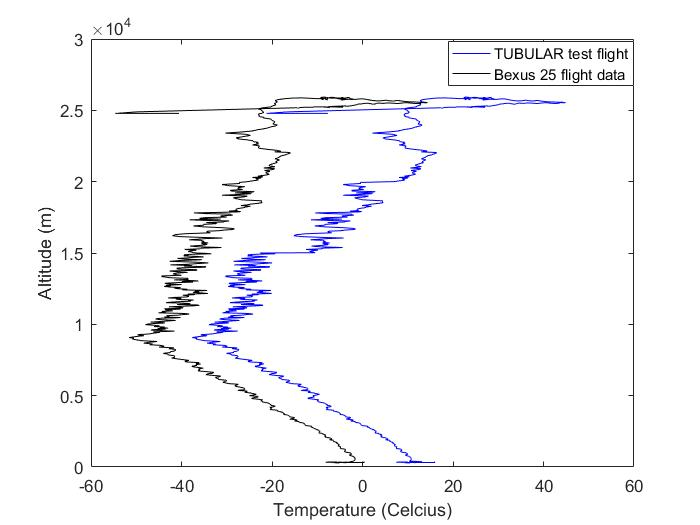
\includegraphics[width=\textwidth]{4-experiment-design/img/Thermal/AAC-test-flight.jpg}
    \caption{Simulated Test Flight AAC}
    \label{fig:test-flight-AAC-4-6}
\end{figure}

The following two figures in Figure \ref{fig:Pump-Valve-ascent-sample-4-6} are a visualization of the pump and the manifold at the time in which the AAC sampling begins during ascent. 
\begin{figure}[H]
    \centering
    \subfloat{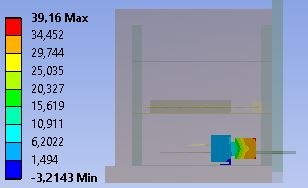
\includegraphics[width=0.45\linewidth]{4-experiment-design/img/Thermal/Pump-sampling-with-box}}
    \hifll
    \subfloat{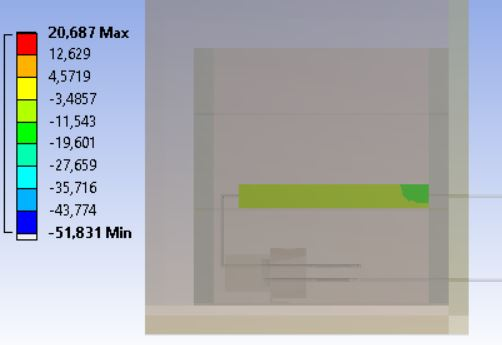
\includegraphics[width=0.45\linewidth]{4-experiment-design/img/Thermal/valve-sampling-with-box}}
    \caption{Pump and Manifold at the Time to Sample During Descent}
    \label{fig:Pump-Valve-ascent-sample-4-6}
\end{figure}

During a worst case simulation that is shown in Figure \ref{fig:Pump-Valve-ascent-sample-4-6} the three heaters were used for 57.5 Wh in total together over the course of the simulation. Only the pump heaters might require more time if it is colder outside and there is dedicated 80 Wh in the power budget table, Table \ref{tab:power-design-table}. So there is a margin to keep the pump heaters on for a longer time if needed.

Based on the calculations and thermal simulations, it can be concluded the thermal designed passive and active thermal control mechanisms detailed in this section will ensure that the AAC's pump and manifold will operate nominally during the entire flight flight. It has been concluded that the CAC has a sufficiently adequate thermal design to operate throughout the whole flight.